\chapter{The Fundamentals of Resilience in Cloud Computing}
\label{ch:resillience}
\textit{The previous chapter introduced cloud computing and how we can utilize it when deploying and managing our software. This chapter describes the fundamentals of system resilience in order to understand the relationship between dependability and adaptivity. Both terms are subcomponents of resilience, and it is therefore necessary to define both terms and their subcomponents in order to analyse their correlation.}

Nygard describes how software engineering is taught incompletely, and that the focus when developing distributed software should be shifted. Nygard states that focus should be laid on what a system should not do, contra today's focus on what a system should do. The first acknowledgement when developing distributed systems is according to Nygard the realisation that failure will occur, and focus should be laid on handling them instead of avoiding them altogether. Further stating that a stable system will keep on working as intended, even though persistent stress or component failure is present. Nygard states the following \cite[p. 27]{nygard2007release}:

\tquote{Once you accept that failures will happen, you have the ability to design your system's reaction to specific failures. [..] This sort of self-protection determines the whole system's resilience}{Nygard}{2007}

Strigini describes a movement within information and communication technology, stating that newly developed systems are more interconnected and changed without global system intervention by developers. Setting unprecedented requirements to existing practices of dependable design, making current practices inadequate when trying to deliver satisfactory levels of dependability \cite[p. 5]{strigini2012fault}:

\tquote{While existing practices of dependable design deal reasonably well with achieving and predicting dependability in ICT systems that are relatively closed and unchanging, the tendency to making all kinds of ICT systems more interconnected, open, and able to change without new intervention by designers, is making existing techniques inadequate to deliver the same levels of dependability}{Strigini}{2012}

Dealing with resilience in distributed systems is a necessity when applications are growing in scale and complexity. The following chapter will establish a definition of resilience which can be used to evaluate application and infrastructure architecture. 

\section{Defining Resilience}
Resilience stems from the Latin word resilíre, meaning "to leap back", the Oxford dictionary defines resilience as the capacity to recover and spring back into shape:

\defi{Resilience (Oxford)}{1. the capacity to recover quickly from difficulties; toughness. \\ 2. the ability of a substance or object to spring back into shape; elasticity.}{\url{https://en.oxforddictionaries.com/definition/resilience}}

Relating resilience to software engineering can be defined as a system's ability to "bounce back" and adapt to disruption \cite{omer2013resilience}. Resilience has been used within many disciplines before being applied to software engineering and has been defined very broadly, potentially incorporating many aspects within cloud computing. The following section will try to pin down what resilience means within cloud computing and what it entails to strive for a system with a high resilience.

Resilience has been defined and characterised by many different parties, within several disciplines \cite{folke2002resilience, dalziell2004resilience, rose2005modeling, andersson2006urban, fiksel2003designing, bruneau2003framework, reed2009methodology, pavard2006design}.
These definitions help understand the meaning of resilience and link it to the understanding of cloud computing. Important keywords from these definitions have been identified, creating an overview of different resilience characteristics. The keywords identify the core concepts that resilience convey when used, all very relevant when defining resilience within cloud computing.

All collections of keywords relate very closely, and help define key concepts within resilience with keywords such as: \textit{stable equilibrium, cope, adapt, proactive measures, reorganize, retain structure, redundancy, robustness}. The context in which there is a necessity for resilience is also included and clear, focusing on the possible disruptive events, described with the following keywords: \textit{undergoing change, face of disruption, face of stress, perturbation, disruptive events}, emphasizing the need for resilient systems in environment characterized by these keywords.

The keywords can be grouped and related to known principles within cloud computing, making it possible to identify resilience characteristics in cloud computing, creating a model for a cloud computing related resilience definition. The keywords were grouped according to their association, and a headline for each group was defined, inspired directly by the identified resilience keywords and known cloud computing keywords. The resilience model is seen in Figure \ref{fig:resilience_keywords_grouped}. The two overarching words being \textit{dependability} and \textit{adaptivity} each with several sub-concepts.

\begin{figure}[!htb]
\begin{center}
  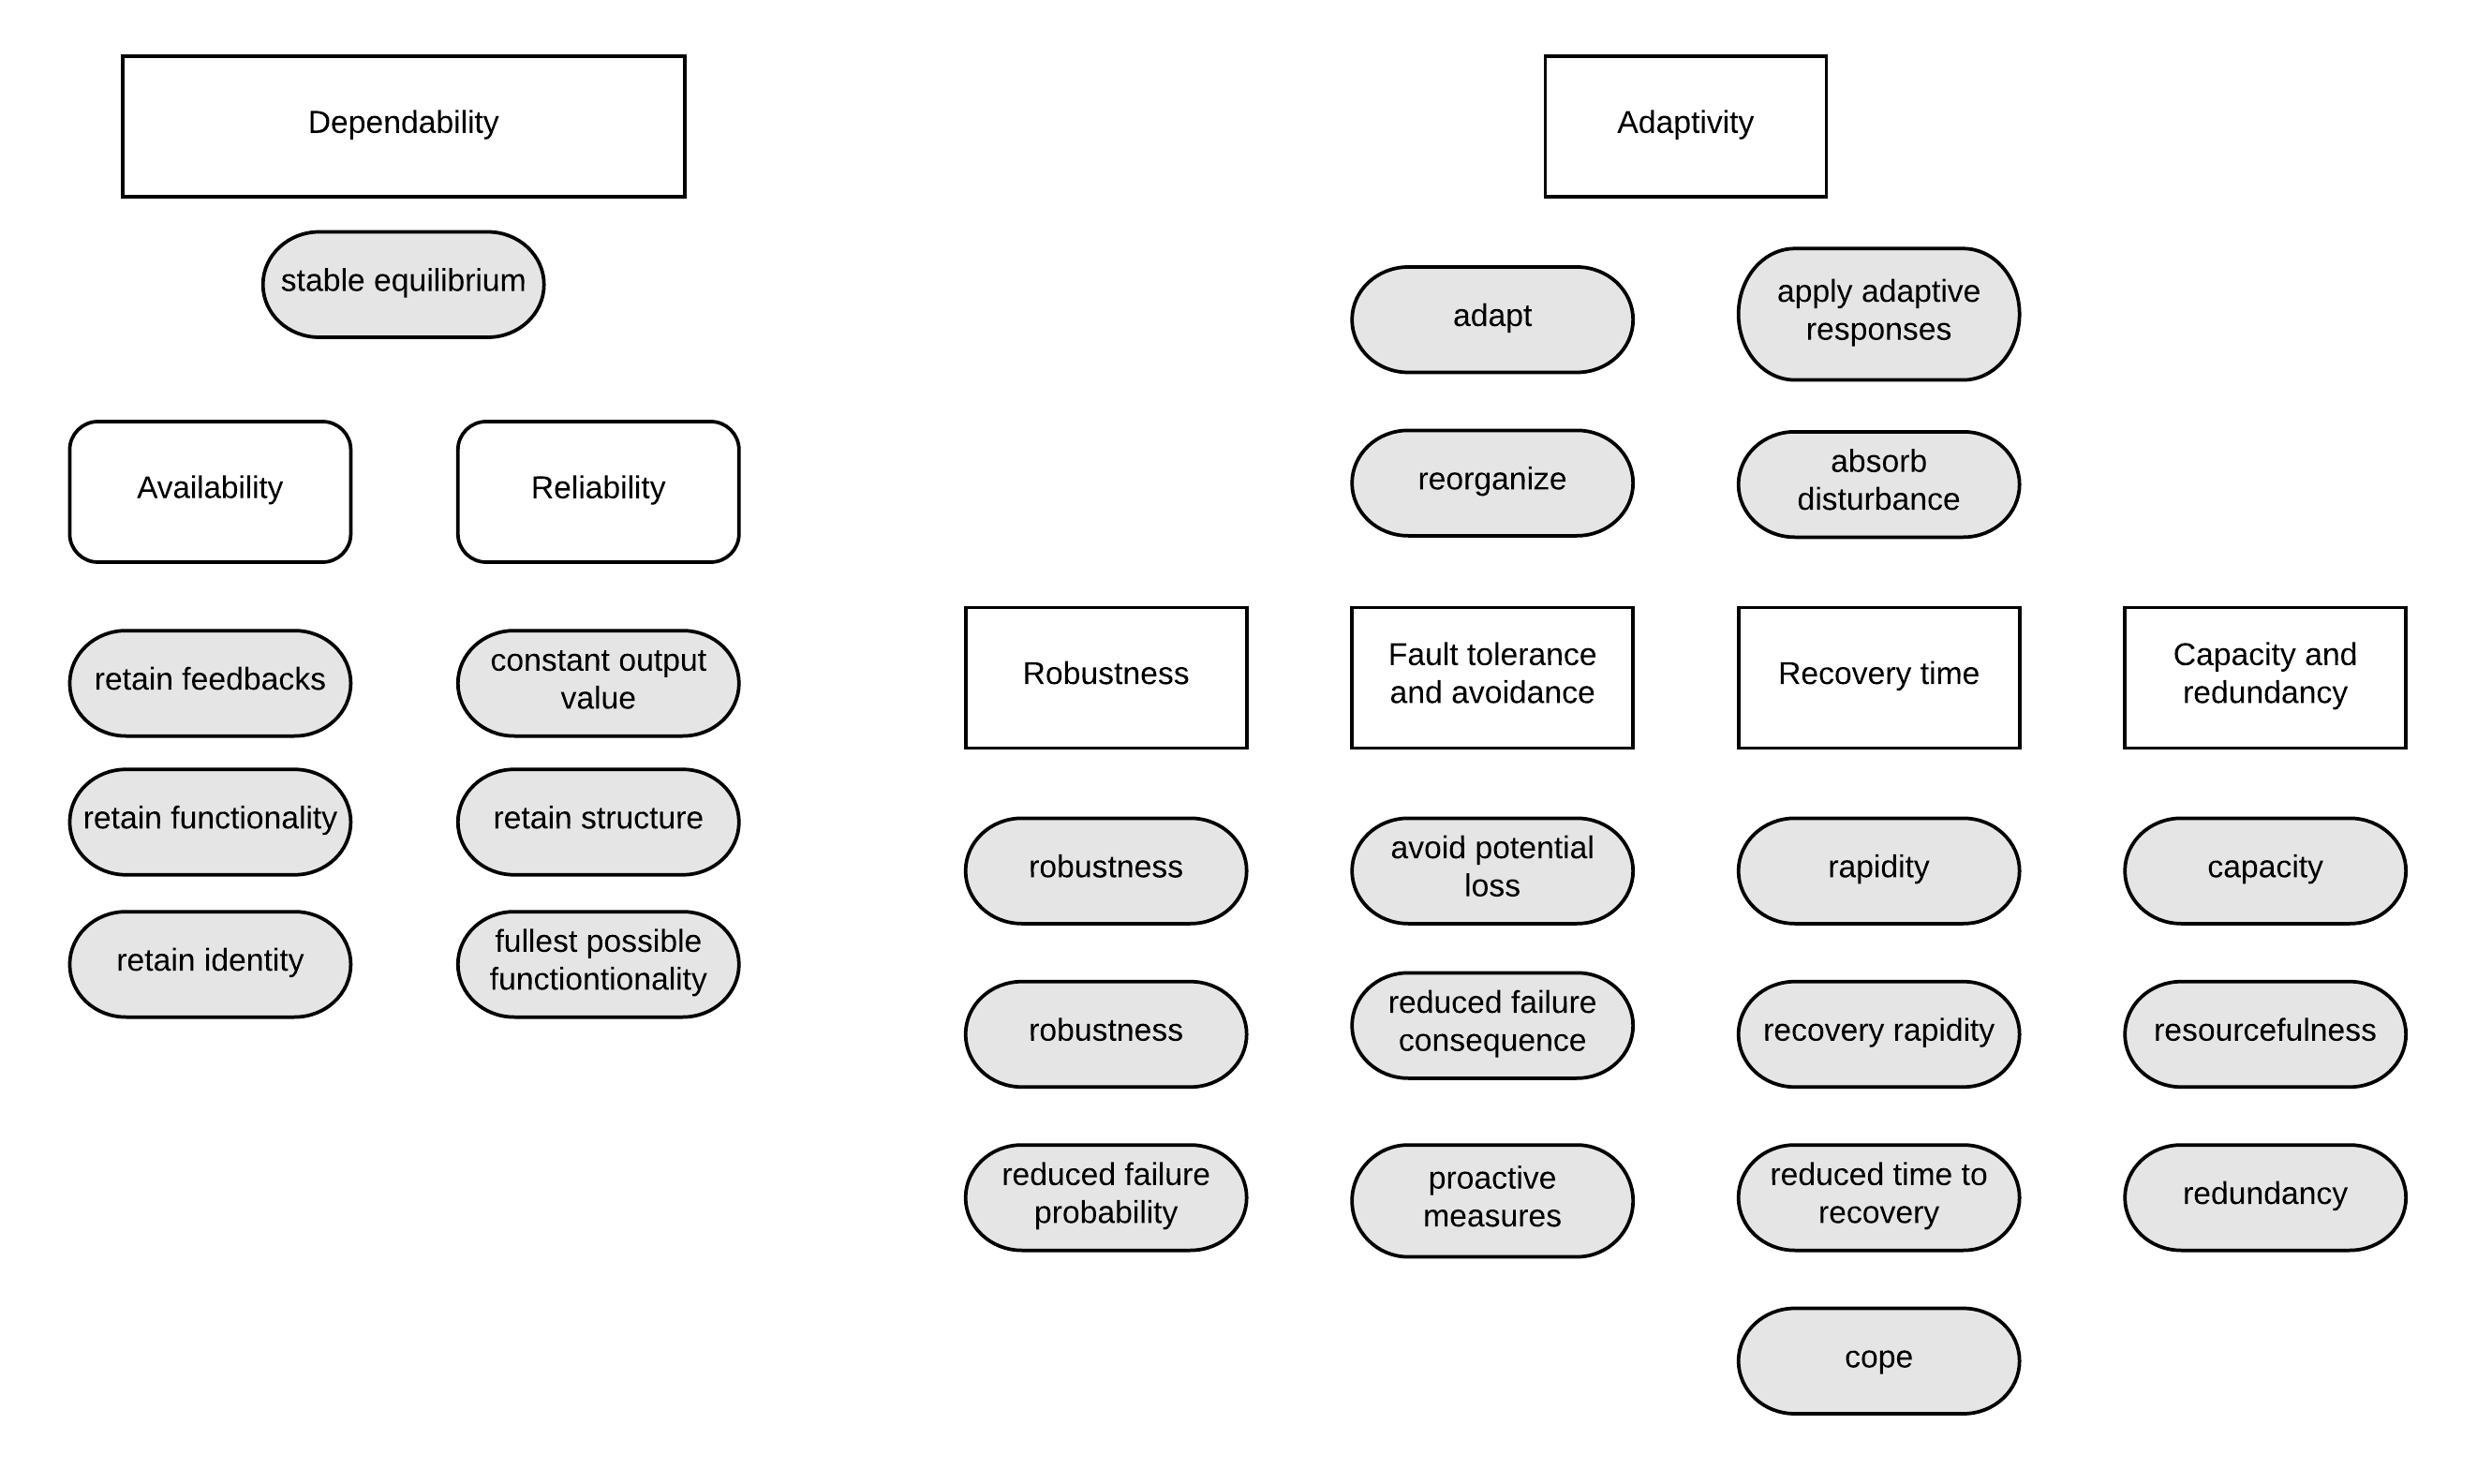
\includegraphics[width=\textwidth]{resilience_keywords_grouped}  
  \caption{Resilience keywords grouped in a cloud context}
  \label{fig:resilience_keywords_grouped}
 \end{center}
\end{figure}


\section{Dependability}
Dependability describes the system's ability to deliver the intended level of service, and therefore whether the service is reliable. Having a dependable service means to have a service level that is not impacted by faults and their derived errors. Dependability makes it possible to quantify how resilient a given system is.

A service state fluctuates between service accomplishment and interruption, the overall goal is too keep the service at the expected service level. The transition between these states is controlled by restoration and failure events, either pushing the service in a direction that aligns or deviates with the intended service level illustrated in Figure \ref{fig:resilience_definition_dependability}. Dependability is mainly quantified through measures on \textit{availability} and \textit{reliability} \cite{laprie1985dependable}.

\begin{figure}[!htb]
  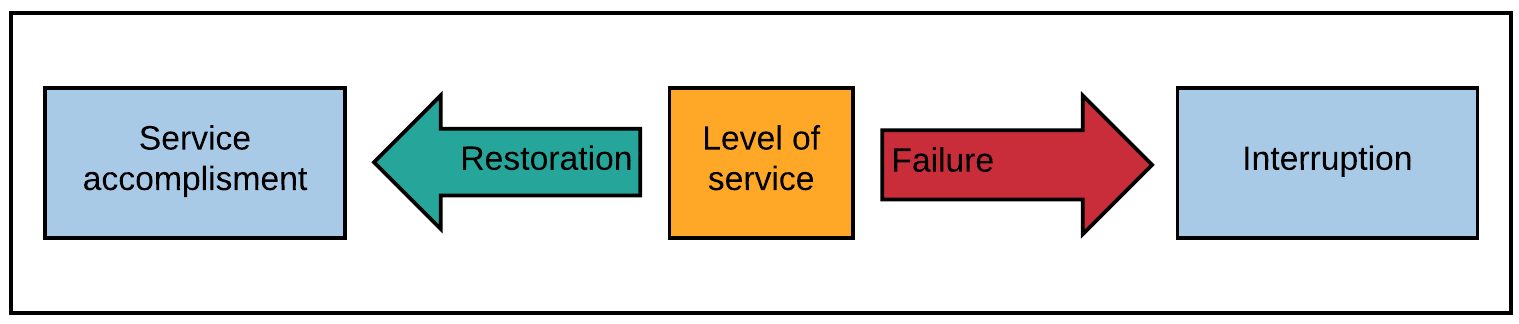
\includegraphics[width=\textwidth]{resilience_definition_dependability}  
  \caption{The service level alternating between service accomplishment and interruption}
  \label{fig:resilience_definition_dependability}
\end{figure}


\subsection{Availability}
Availability describes the accessibility to a given service, and is generally determined by calculating the time a service was unavailable over a given period. The availability level can be determined by stating how much downtime is allowed within a given period \cite[p. 477]{beyer2016siteReliabilityEngineering}. If a service times out and does not present an error message it is considered unavailable. A service only exists, from the user's perspective, if it is available \cite[p. 345]{beyer2016siteReliabilityEngineering}. 

Google describes how they measure service risk across their entire infrastructure by evaluating \textit{unplanned downtime}  \cite[p. 26]{beyer2016siteReliabilityEngineering}. According to Beyer et al. there are two ways of measuring service availability, Time-based and Aggregate availability. Time-based focuses on the accepted level of unplanned downtime, usually expressed in the number of 'nines' (eg. 99.999\%), this is often calculated on the proportion of a services uptime. Aggregate availability on the other hand focuses on request success rate, due to Google's infrastructure always being 'partially' functional. Aggregate availability makes it easier to apply availability measurements to services that only run part-time.

\begin{figure}[!htb]
  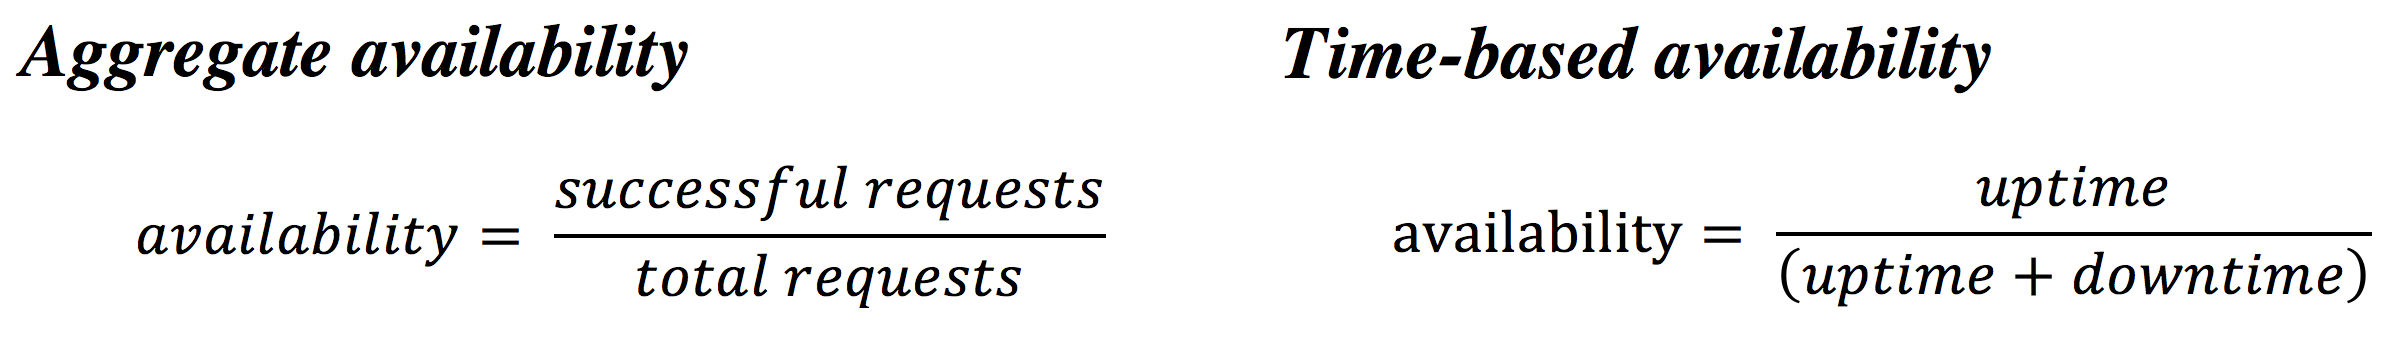
\includegraphics[width=\textwidth]{resilience_definition_availability}  
  \caption{Aggregate and Time-based availability equations}
  \label{fig:resilience_definition_availability}
\end{figure}

Google sets availability targets for all their services, comparing the performance to a defined goal and fixing deviations as they arise.

\subsection{Reliability}
Reliability is the probability that a system will fulfil set requirements in stated conditions for a given period of time \cite{o2012practical}. The resilience of the system therefore determines the reliability by analysing the amount of external disruption a system can handle. Google states that reliability is the fundamental feature of a system, and autonomous and resilient system behaviour is a good way to achieve reliability \cite[p. 84]{beyer2016siteReliabilityEngineering}.

\section{Adaptivity}
Adaptivity can be defined as the system's ability to adapt to a disruptive situation and reconfigure themselves, without loss in the intended level of service, including the ability to adjust to changing internal demands \cite{reed2009methodology}. Adaptivity consists of different measures that can be actively improved by design. By designing a system that takes either of the adaptivity subcomponents into account, the dependability is increased, thereby increasing resilience. Adaptivity consists of: \textit{Capacity and redundancy}, \textit{Robustness}, \textit{Fault tolerance and avoidance} and \textit{Recovery time}.

\subsection{Capacity and Redundancy}
Capacity and redundancy are two different aspects that inherently are very linked. Capacity is the highest throughput a system can deliver, with and acceptable response time for each request \cite[p. 136]{nygard2007release}. Redundancy meaning how much excess capacity a system has that can be applied in case of failure to uphold stated system requirements.

Capacity and redundancy can be used on a service basis, using capacity to denote the total number of services running, whereas redundancy denotes the number of excess services currently running. Load can either be distributed across all services at all times, or served form a primary services, here the redundancy services are used as backup services, in case the primary service fails.

\note {
\begin{figure}[!htb]
  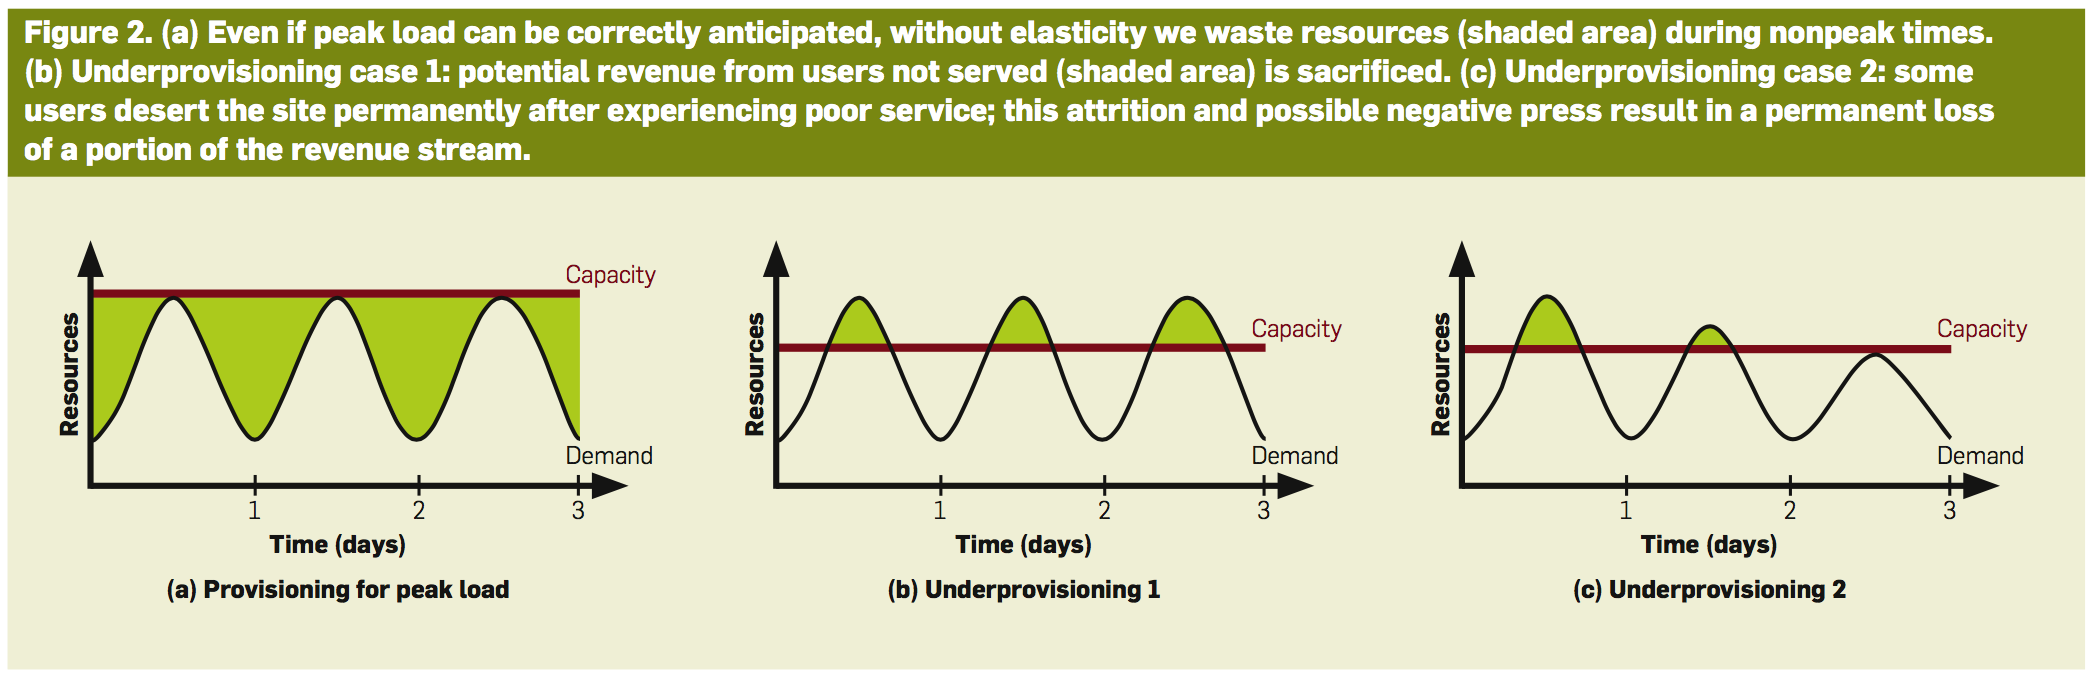
\includegraphics[scale=0.15]{resilience_capacity}  
  \caption{Capacity figure from: Ambrust et al. – A View of Cloud Computing \comment{Make own picture of this :).}  }
  \label{fig:resilience_keywords_grouped}
\end{figure}
}
\subsection{Robustness} 
Robustness covers how quantifiable the system behaviour is in the face of disruption challenging system behaviour \cite[p. 10]{sterbenz2010resilience}. These disruptions are both internal and external \cite{omer2013resilience}. Robustness includes the system's ability to withstand disruptions rather than adapt to them, a robust system has been designed to withstand known uncertainties, maintain intended level of service and same form of functionality.

\note {
\comment{Kig på: "Evaluating robustness of cloud-based systems" Godt input til robustness}
}

\subsection{Fault Tolerance and Avoidance}
Fault tolerance and avoidance is used to describe dependability of a system, from internal and external harm. Tolerance is making the system tolerable to the effects of faults. Avoidance meaning guarding a system against potential defects that could cause system failure \cite{strigini2012fault}.


\subsection{Recovery Time} 
Recovery time is a measure for how long time period a system needs to resume fulfilling the stated requirements.

\section{The Availability and Capacity and Redundancy Relationship}
Dependability and adaptivity are inherent very linked which in turn means that the same is present for Availability and Capacity and Redundancy. If a adaptivity improving design is utilized the dependability of the system will increase. Improving capacity or introducing redundancy will increase the attainable throughput with which a service can deliver a satisfactory availability.

An example is shown in Figure \ref{fig:resilience_aggregate_avalability_example} where the loss of a single node reduces the capacity and therefore gives a suboptimal availability.

\begin{figure}[!htb]
  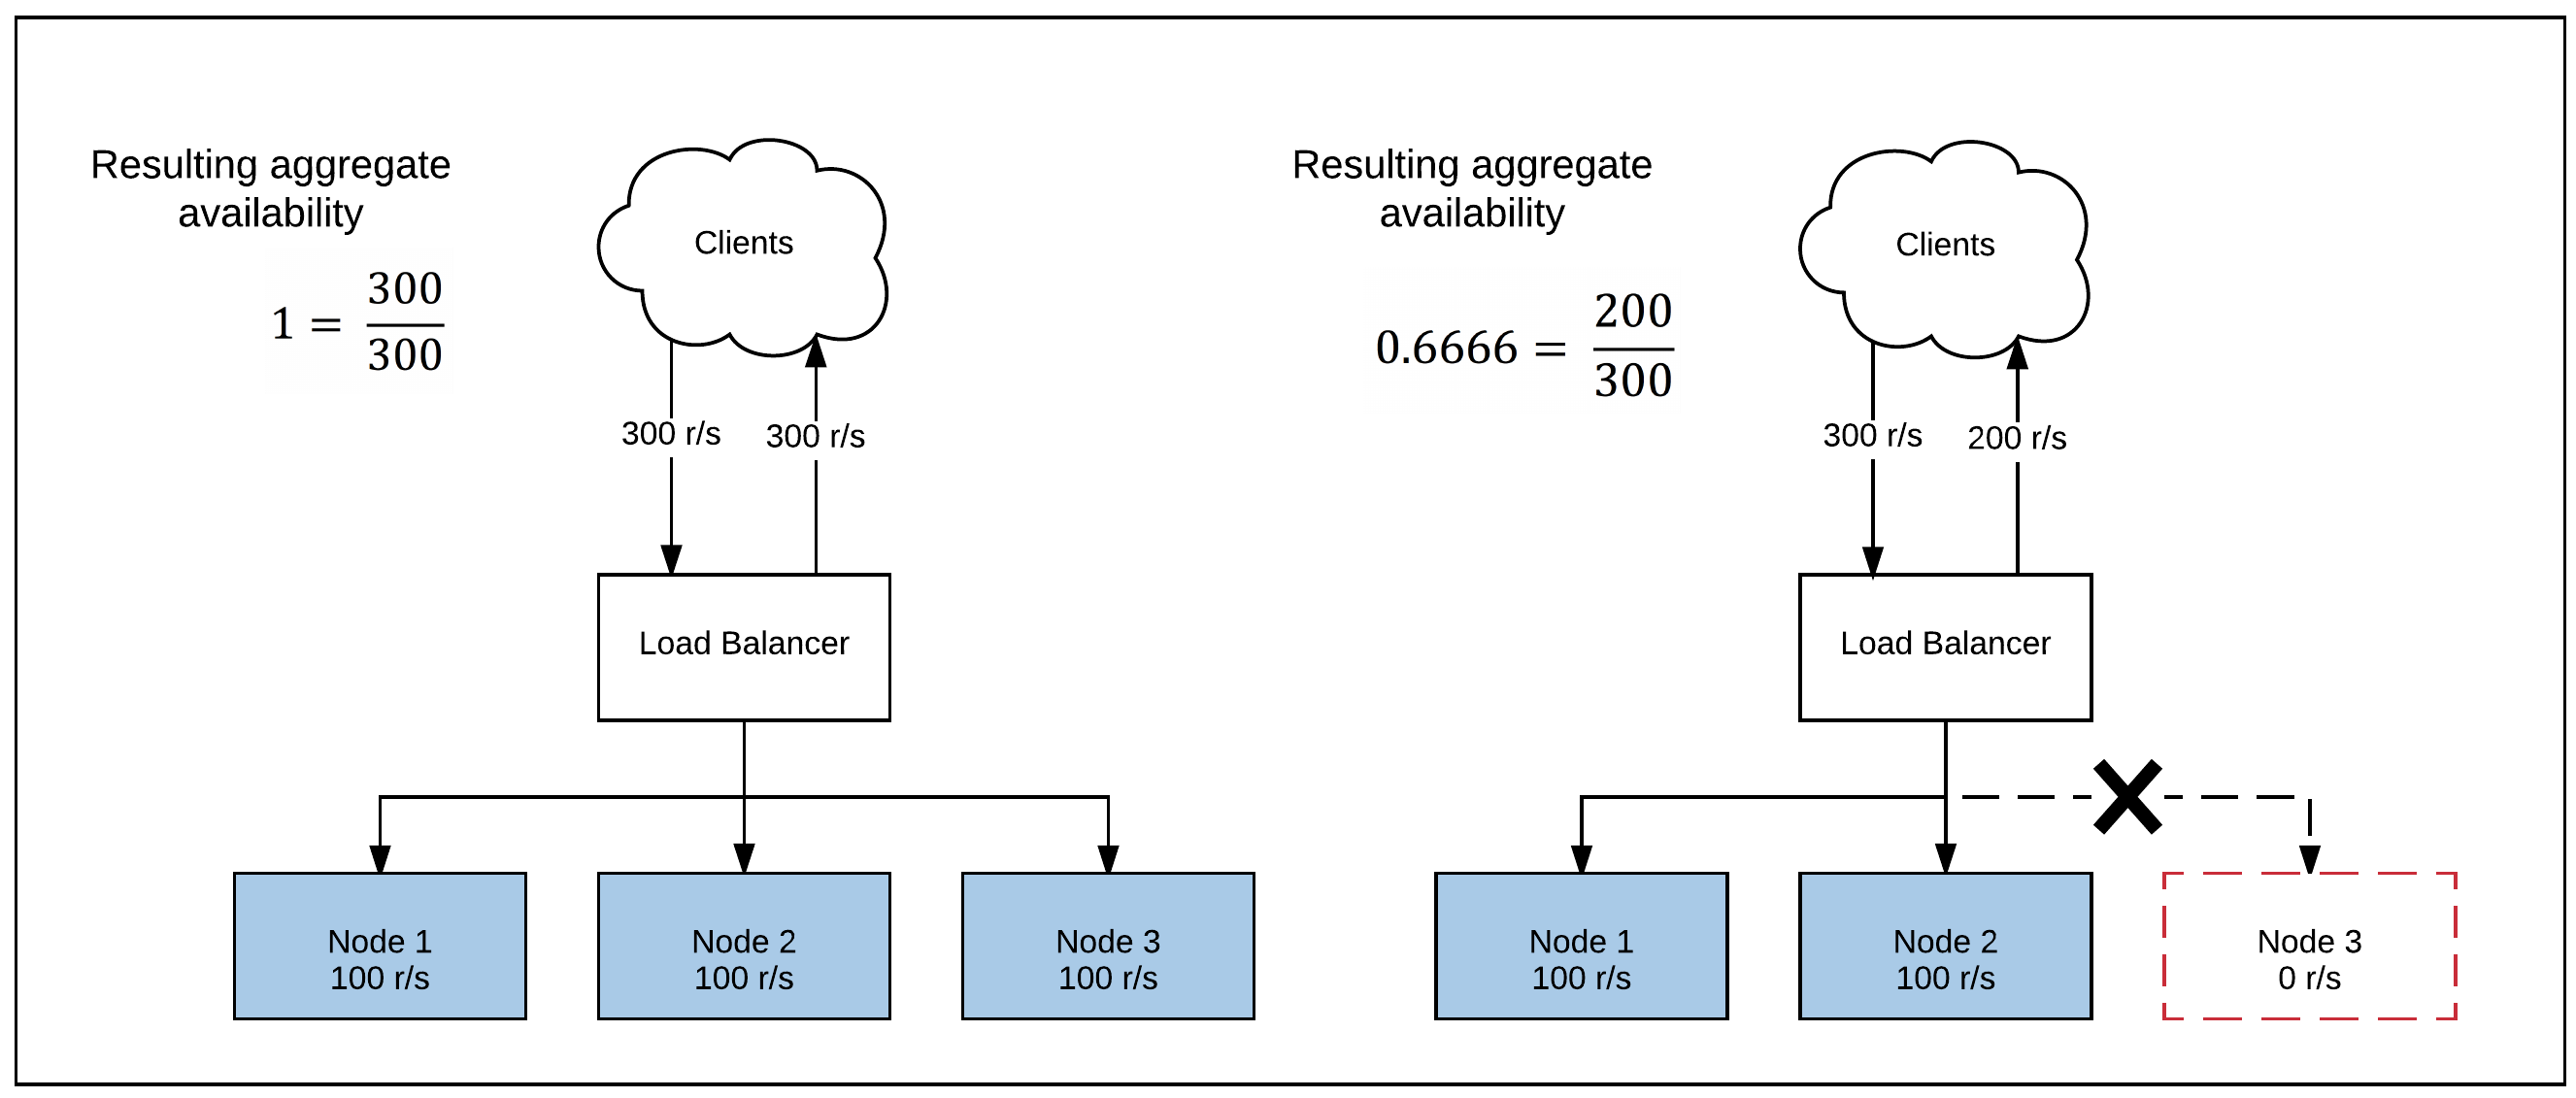
\includegraphics[width=\textwidth]{resilience_aggregate_avalability_example}  
  \caption{An example showing an aggregate  availability calculation. Availability is decrease due to a lack of capacity}
  \label{fig:resilience_aggregate_avalability_example}
\end{figure}

The availability in this example is calculated for a expected 300 requests per second, to uphold an availability of 1 a capacity of 300 request per second is required. Without any redundancy in place a single failing node means that the availability will be reduced, in turn reducing the systems resilience. 

There are several known patterns that help increase system resilience, and several antipatterns that are known to reduce a systems resilience. They will be described below to understand how resilience in a distributed system is improved.

\section{Stability Antipatterns}
\label{sec:stability_antipatterns}
When working with big complex systems, rest assure: Failure is bound to happen. How the failure was triggered, which fractures it created and how much it propagated will differ each time. Stability antipatterns is a concept Nygard uses when understanding how these failures appear within a distributed system, which characteristics the failures have and how some architectures lead to them \cite[p. 31]{nygard2007release}.

\subsection{Integration Points}
Integration points are connections from a service to other services, necessary for the service to deliver expected functionality. Nygard denotes integration points as the: "The number-one killer of systems" \cite[p. 33]{nygard2007release}. Integration points often run over socket connections which are not immediate and incur complexity. Many simultaneous connections can hamper a remote application, forcing the calling application to wait, and possible decrease service level.
Circuit breakers, decoupling middleware and testing can help solve or identify challenges with integration points.

\subsection{Chain Reactions}
Chain reactions can form if one of several serving servers fail, and therefore inflict a higher load on the remaining running servers. If one server has failed because of an internal error, load is increased on the remaining servers, also containing internal errors, increasing the probability of similar errors happening in the remaining servers. Typical errors include resource leaks and obscure race conditions.
Server bulkheads prevent chain reactions from depleting entire services, circuit breakers protect caller services.

\subsection{Cascading Failures}
Cascading failures happen when a failure from one layer cause problems in callers. If a failure happens in a serving service and callers are not correctly handling it (eg. implementing a time-out), the failure can cascade into the calling service. Nygard calls cascading failures "the number on crack accelerator" \cite[p. 49]{nygard2007release}.
The circuit breaker pattern and timeouts can combat cascading failures.

\subsection{Users}
Users increase the amount of traffic, and will eventually surpass capacity, unless increased with a growing demand. If a transaction is too long, the demand has surpassed the capacity. Derived errors can occur if the capacity is fully utilized, for example memory exhaustion, causing other internal services to fail. These derived errors can be combated with a correct service capacity.

\subsection{Blocked Threads}
Concurrency errors within a service can block several threads. Timeouts in wait functions can defend against indefinitely blocked threads.

\subsection{Attacks of Self-Denial}
Attacks of self-denial is never a system error, but is caused by the people around the system. Nygard describes situations where advertisement campaigns has created big spikes of sudden and unforeseen load that takes the system down due to insufficient capacity. 
Either a "shared-nothing" architecture, decoupled middleware or horizontally scaling of the shared resources required in the advertisement campaign can mitigate self-denial attacks. A "shared-nothing" architecture encapsulates the entire service within a single server, making it linearly scalable, combating huge load spikes and isolating possible failures.

\subsection{Scaling Effects}
Scaling effects describe the effects of a system handling increasing amounts of load, previous sufficient capacity levels become insufficient. Test environments often do not show scaling effects due to their limited scale.
Scaling effects can be negated by avoiding internal point-to-point communication and stress testing shared resources, implementing proper fallback behaviour if they fail.

\subsection{Unbalanced Capacity}
Unbalanced capacity refers to the service capacities of dependent services and their balance. Capacity variance between development and deployment environments and what potential fallacies this can introduce. Unbalanced capacity can introduce scaling effects, where one service scales accordingly whereas another, dependent service capacity, remains stagnant.

\subsection{Slow Response}
A quick response lets the calling service proceed rapidly, a slow response, on the other hand, ties the resources that the calling service is using for a longer period. Slow responses can trigger cascading failures, due to slow upstream responses from a calling service that is tied up in a slow response. Slow responses cause increased amounts of traffic due to users' frequently reloading pages loading slowly. Slow responses can be solved by failing fast if response times exceed upper timing limits, and ensuring that there is not a shared resource contention.
A slow response ties up the resource on the calling end, the longer a call is on a service provider, the larger the caller needs to scale in order to handle the same amount of traffic.


\subsection{SLA Inversion}
Service-level agreement inversion is when a service promises a specific service level without taking into account the service-level agreement of the services it relies on. Service-level is determined by the dependencies service-levels and the probability for failure internally. It is therefore important to decouple from dependent services and degrade functionality gracefully as dependant services fail. If decoupling is not possible, circuit breaks can be put into place. 


\subsection{Unbound Result Sets}
Unbound results sets occur when the amount of requested data is not limited, and the result set therefore grows equally with the entire data set. Limiting the result set will ensure that memory in the calling application will not be exhausted if the data set is expanding.


\section{Stability Patterns}
Stability patterns are applied to increase stability and reduce damage done when errors occur. These patterns serve as design guidance when implementing services.


\subsection{Timeouts}
Network connections are slow and error prone, but necessary to incorporate in any distributed application. Applying timeouts at integration points help avoid blocked threads and mitigate slow responses from dependent services. By defining timeouts an upper limit for time waiting is set, and the application can then move on and recover from failure.


\subsection{Circuit Breaker}
The circuit breaker pattern is based on the principles and functions of a fuse in electric circuits. From a software perspective, the idea is to wrap dangerous operations, so that they can be circumvented when not working properly. This allows a system to degrade functionality if errors occur, guarding against integration points, slow responses, unbalanced capacities and cascading failures.

The circuit break is a state machine pattern, moving between three states: open, closed and half-open. When in open state, requests are processed ordinarily. When in closed state, requests fail immediately. The circuit break can transit from open to closed if requests unexpectedly are unsuccessfully processed. The half-open state processes requests ordinarily to test if it is possible to process requests successfully. If requests are processed successfully in the half-open state, the circuit breaker changes the state to open. A threshold specifies the amount of unsuccessful processed requests that triggers state transition from open to closed state. Another threshold determines when to transit from closed to half-open state.

Circuit breaker guards against integration points, and when a failure occurs in a integration point, it should not be called. Used together with timeouts, that can inform the system of a present error.

\subsection{Bulkhead}
The bulkhead design pattern is inspired by bulkheads known from ship design, where compartments throughout the ship divides the ship into watertight partitions. This ensures that a single penetration of the ship's hull does not sink the ship. When applied to software, bulkheads are used to partition capacity, preserving functionality if errors occur. Bulkheads can protect against chain reactions, by ensuring backups of services important to several other services. The bulkhead pattern is usable on both an application and infrastructure level, by partitioning thread pools, server CPU or separate servers, determining the granularity. 


Bulkheads are excellently implemented with virtualization, where capacity can be changed quickly by increasing or decreasing the allocated amount of independent services.

\subsection{Steady State}
Steady state refers to intended state of a service, where the functionality is completely fulfilled and the service is operating as intended. Many factors influence this steady state and some potentially interrupt it. Manual operations incur overhead and eventually introduce human made errors, a system should be able to run indefinitely without operational intervention. 
Further more mechanism that accumulates resources must be drained at the same rate or greater not to overflow. When mechanism overflow, errors can occur by increasing response time or slowing down databases. By purging unused data from databases, clogging of server memory is avoided, which could potentially slow read and write operations. Log files are also a potential memory clog, and should therefore be left of the production server.

\subsection{Fail Fast}
The fail fast principle dictates informing callers quickly when a system SLA cannot be met. By failing fast the system avoids incurring internal problems externally. By verifying that integration points are correctly working early, potentially wasted resources are reserved by completely avoid running transactions that cannot complete in their entirety.

\subsection{Handshaking}
Handshaking refers to how services accept future workloads from other services. By acknowledging that the service can live up to the stated SLA, and service the required capacity before communication begins, the service can protect itself by throttling incoming requests to serviceable levels. Health checks where a service is checked before calling can spare a standard call that fails.

\subsection{Test Harness}
A test harness is a supplement to traditional unit tests, acceptance test. The test harness job is to emulate remote systems on the other side of integration points, and mimic responses to remote calls on the network. By mimicking the dependencies, developers are able to test how the service reacts to malicious responses of different kinds.

\subsection{Decoupling Middleware}
Decoupling Middleware is the communication protocol used to communicate between dependent but decoupled services. Varying from same time, host and process to different time, host and process.

Nygard describes how fundamental it is to the system design which form of communication is chosen, and how big consequences for the implementation changing this has. Choosing communication in a system is on an architecture level fundamentally changing the implementation of individual services within the system.